\documentclass[acmsmall,10pt,review,anonymous]{acmart}\settopmatter{printfolios=true,printccs=false,printacmref=false}
\usepackage{booktabs,listings,xspace,wrapfig}
\lstset{language=R}
\usepackage{my_style}
\definecolor{LightGray}{rgb}{.95,.95,.95}
\definecolor{Gray}{rgb}{.3,.3,.3}
\definecolor{DarkGray}{rgb}{.5,.5,.5}

\graphicspath{ {./plots/} }

\lstset{ %
  columns=flexible,
  captionpos=b,
  frame=single,
  framerule=0pt,
  framexleftmargin=-1mm,
  framexrightmargin=-1mm,
  tabsize=2,
  belowskip=0pt,
  basicstyle=\small\ttfamily,
  backgroundcolor=\color{LightGray},
  emphstyle=\sffamily,
  keywordstyle=\bfseries,
  commentstyle=\color{Gray}\em,
  stringstyle=\color{Gray},
 % numbers=left
}

\lstdefinestyle{R}{ %
  language=R,
  deletekeywords={env, equal, c, runif, trace, args},
  breaklines=true
}

\lstdefinestyle{Rin}{ %
  style=R,
  numberstyle=none,
  basicstyle=\normalsize\ttfamily,
  breaklines=false
}

\newcommand{\code}[1]{\lstinline|#1|\xspace}
\newcommand{\genthat}{{\sc Genthat}\xspace}

\setcopyright{none}
%\setcopyright{acmcopyright}%\setcopyright{acmlicensed}
%\acmDOI{10.475/123_4}
%\acmConference[OOPSLAs]{Woodstock conference}{July 1997}{El Paso, Texas USA}
%\acmYear{1997}%\copyrightyear{2016}%\acmPrice{15.00}
\begin{document}

\title{A Large-scale Study of Polymorphism in R}

\newcommand{\PACKAGES}{11,463\xspace}
\newcommand{\PROGRAMMERS}{?\xspace}
\newcommand{\PERCENTCRAN}{83\%\xspace}
\newcommand{\CRANTOTAL}{13,841\xspace}
\newcommand{\RLOC}{15,050,267\xspace}
\newcommand{\CLOC}{9,373,542\xspace}
\newcommand{\YEARS}{?\xspace}
\newcommand{\INDEXCOINCIDENCE}{3,499\xspace}
\newcommand{\TOTALINDEXY}{6,561\xspace}
\newcommand{\INDEXYPERC}{53\%\xspace}		% TODO Not an accurate count.
\newcommand{\DATAPKGS}{206\xspace}
\newcommand{\DATAPKGSPERC}{1.5\%\xspace}
\newcommand{\METAARGCOUNT}{7,051\xspace}

\begin{abstract}
The R programming language is widely used in a variety of scientific domains
for tasks related to data science. The language was designed to favor an
interactive style of programming with minimal syntactic and conceptual
overhead. This design is well suited to support interactive data analysis,
but is not well suited to generating performant code or catching programming
errors.  In particular, R has no type annotations and all operations are
dynamically checked at runtime. The starting point for our work is the
question: \emph{what could a static type system for R look like?}  To answer
that question we study the polymorphism that is present in \RLOC lines of R 
code spread among some \PACKAGES packages, written over a
period of over \YEARS years by \PROGRAMMERS programmers.  We perform a dynamic
analysis, leveraging tests and use-cases, to determine the level of
polymorphism that is present in the code. We do this for several potential
notions of types. Our result suggest that polymorphism is important in some
key parts of the system but that relatively simple type annotations could be
used to capture most of the interesting cases.
\end{abstract}

\maketitle

\section{Introduction}

Our community builds, improves, and reasons about programming languages.  To
make design decisions that benefit most users, we need to understand the
language we are working with as well as the real-world needs it
answers. Often, we, as researchers, can appeal to our intuition as many
languages are intended to be general purpose and appeal to users with some
computer science training. Unfortunately, these intuitions don't always
apply to domain-specific languages, languages designed for and by a specific
group of users to solve very specific needs. This is the case of the data
science language R.

R and its ancestor S are languages designed, implemented and maintained by
statisticians. Originally they were designed as glue languages, languages
that would allow to read data into vectors and call statistical routines
written in Fortran. Over three decades, the languages became widely used
across many fields of science and in industry for data analysis and data
visualization; with time additional features were added.  Modern R, as a
linguistic object of study, is fascinating. It is a vectorized, dynamically
typed, lazy functional language with limited side-effects, extensive
reflective facilities and retrofitted object-oriented programming support.

Many of the design decisions that gave us R were intended to foster an
interactive, exploratory, programming style. This includes, to name a few,
the lack of type annotations on variables and functions, the ability to use
syntactic shortcut, and the automatic conversion between data types.  While
these choices have led to a language that is surprisingly easy to use by
beginners --many data science programs do not teach the language itself but
simply introduce some of its key libraries-- they have also created a
language where almost all computations yield a numeric result and where
errors can go undetected. 

One way to increase assurance in the results obtained when using R would be
to add type annotations to functions and variable declarations. These
annotations could then be used, either statically or (more likely)
dynamically, to catch mismatches between expected and provided data values.
The nature of R is such that it is unlikely to be ever fully statically
checked, furthermore end users may not be willing to write types when
carrying out exploratory programming tasks. So, we are looking for an
optional type system that would allow us to capture as much of behavior of
library functions as possible while remaining easy to understand for
end-users and library developers alike.

This papers is a data-driven study of what a type system for the R language
could look like. Longer term, our intention is to propose changes to
language, but for any changes to be accepted by the user community, they
must clearly benefit the language without endangering backwards
compatibility. Our goal is thus to find a compromise between simplicity and
usefulness; the proposed type system should cover most common programming
idioms while remaining easy to use. In order to do this, we need to
understand the degree of polymorphism present in R code, that is to say, how
programmers leverage the dynamic nature of R to write code that can accept
arguments of different types.  This understanding will drive our design.

We propose to capture the degree of polymorphism present in R by the means
of a dynamic analysis of widely used libraries. For each function call we
can record the types of its arguments and of its return value. This allows
us to observe how many different combination of types are accepted by any
given function. Unlike many other languages, R has a carefully curated
software repository called CRAN. To be deposited in CRAN, a package must
come with sample dataset, tests and executable use-cases. As part of normal
operations these tests are run regularly and failing packages are removed.
This allowed us to have access to \PACKAGES libraries and about an order of
magnitude more runnable scripts that exercise those libraries.

The contributions of this paper are thus as follows:
\begin{itemize}
\item A large-scale analysis of the polymorphism present in function
  signatures of \PACKAGES widely used and actively maintained R packages.
\item A tracing and analysis pipeline that extends a previously published
  test generation tool named \genthat.
\item Manual analysis of 100 functions to validate the dynamic analysis
  results.
\end{itemize}

One threat to validity of our work is that we rely on dynamic analysis, so
our conclusions are only as good as the coverage of the possibly function
behaviors. Previous work~\cite{issta18}, reported that running all the
scripts that come with CRAN packages gives, on average, 68\% test coverage.
We attempted to mitigate the threat coming from the fact that only part of
the code is being exercised by manual analysis. It would be reasonable to
ask for confirmation of the data by static analysis of the code, but sound
static analysis of R is difficult because of the extensive use of reflective
features such as \code{eval} and of the ability to redefine the meaning of
operators such as \code{+} and \code{if}.  Another threat to validity is
that we only have access to code that has been deposited in the CRAN
repository. While this may bias our findings towards code written to be
reusable and, possibly, better engineered than typical user code. This is
also the code that would most benefit from type annotations.

\newpage  %%Leave here

\section{The R Programming Language}\label{sec:rlang}

Over the last decade, the R Project has become a key tool for implementing
sophisticated data analysis algorithms in fields ranging from Computational
Biology~\cite{R05} to Political Science~\cite{R:Keele:2008}. At the heart of
the R project is a \emph{vectorized, dynamic, lazy, functional,
  object-oriented} programming language with a rather unusual combination of
features~\cite{ecoop12} designed to ease learning by non-programmer and
enable rapid development of new statistical methods.  The language, commonly
referred to as R was designed in 1993 by Ross Ihaka and Robert
Gentleman~\cite{R96} as a successor to S~\cite{S88}.  First released in
1995, under a GNU license, R rapidly became the lingua franca for
statistical data analysis. Today, there are over 13,000 R packages available
from repositories such as CRAN and Bioconductor.  With 55 R user groups
world-wide, Smith~\cite{eco11} estimates that there are over 2 million
end-users.

As an introduction to R, consider the code snippet in Fig.~\ref{sample} from
a top-level interaction where the user defines a function \code{normSum}
that accepts vectors of integers, logicals, doubles and complex values and
normalizes the vector with respect to its sum and rounds the results. The
function definition does not require type annotations, and all operations
transparently work on vectors of any length and different types.

\begin{figure}[!hb]{\small
\begin{lstlisting}[style=R]
> normSum <- function( m )  round( m / sum(m), 2)
> normSum(c(1L,3L,6L))
[1] 0.1 0.3 0.6
> normSum(c(1.1,3.3,6.6))
[1] 0.1 0.3 0.6
> normSum(c(1.6,3.3,6.1))
[1] 0.15 0.30 0.55
> normSum(complex(r=rnorm(3),i=rnorm(3)))
[1] 0.49+0.21i 0.30-0.18i 0.22-0.03i
\end{lstlisting}}
\caption{Sample R code}\label{sample}
\end{figure}

In R, function can be called with named parameters, R support variable
argument lists, and arguments can have default values. Putting all of these
together consider the following declaration:

\begin{lstlisting}[style=R]
f <- function(x, ..., y=3) x + y
\end{lstlisting}

\noindent
Function \k{f} can be called with a single argument \code{f(3)}, with named
argument \code{f(y=4,x=2)} and with a variable number of arguments,
\code{f(1,2,3,4,y=5)}, all of these calls will return \code{6}.

R has a number of features that are not crucial to the present
discussion. We will mention some of them here for completeness.  In R, data
structures are reference counted and have copy-on-write semantics, thus the
assignment \code{x[12]<-3} results in an update to a copy of \code{x} unless
the reference count on that object is 1.  This semantics gives R a
functional flavor while allowing updating in place within loops (the first
update copies, subsequent updates are performed on the copy). Arguments to
functions are evaluated only when needed, they are bundled in so-called
promises which package the original expression (as an AST), its environment
as well as the result of evaluating the expression. Promises can be
leveraged for meta-programming as it is possible to retrieve the text of a
promise and evaluate that in a different environment.

\subsection{Types of Data}

Before attempting to define a type system for R, we should understand the
different kinds of values that programs operate on.  As we will see
different notions of type may emerge depending on how granular we want to
be.

\renewcommand{\k}[1]{{\tt #1}\xspace}

R has one builtin notion of type that can be queried by the \k{typeof}
function. Over the years, programmers have found the need for a richer type
structure and have added attributes. The best way to think of attributes is
as an optional map from name to values that can be attached to any object.
Attributes are used to encode various type structures. They can be queried
with functions such as \k{attributes} and \k{class}.

\begin{wrapfigure}{r}{6.1cm}
\footnotesize\begin{tabular}{l|l@{}}\hline
\multicolumn{2}{l}{\bf Vectorized data types:}  \\\hline
\k{logical}  & vector of boolean values\\
\k{integer}   & vector of 32 bit integer values\\
\k{double} & vector of 64 bit floating points\\
\k{complex} & vector of complex values\\
\k{character} & vector of strings values\\
\k{raw} & vector of bytes\\
\k{list} & vector of values of any type\\\hline
\multicolumn{2}{l}{\bf Scalar data types:}\\\hline
\k{NULL}  &  singleton null value\\
\k{S4}    &  instance of a S4 class \\
\k{closure} & a function with its environment\\
\k{environment} & a mapping from symbol to value \\\hline
\multicolumn{2}{l}{\bf Implementation data types:}\\\hline
\multicolumn{2}{l}{\k{special},
\k{builtin},
\k{symbol},
\k{pairlist},
\k{promise}}\\
\multicolumn{2}{l}{
\k{language},
\k{char},
\k{...}, 
\k{any},
\k{expression},
}\\
\multicolumn{2}{l}{
\k{externalprt},
\k{bytecode},
\k{weakref}}\\\hline
\end{tabular}\caption{Builtin Types}\label{types}\end{wrapfigure}

Figure~\ref{types} lists all of the builtin types that are provided by the
language. They are the possible return values of \k{typeof}. There is no
intrinsic notion of subtyping in R. But, in many context a \k{logical} will
convert to \k{integer}, and an \k{integer} will convert to \k{double}.  Some
off conversion can occur in corner cases, such as \k{1<"2"} holds and
\k{c(1,2)[1.6]} returns the first element of the vector, as the double is
converted to an integer. R does not distinguish between scalars and vectors
(they are all vectors), so \code{typeof(5) ==} \code{typeof(c(5)) ==
  typeof(c(5,5))} \code{ == "double"}. Finally all vectorized data types have a
distinguished missing value denoted by \code{NA}. The default type of
\code{NA} is \k{logical}. We can see that \code{typeof(NA)=="logical"}, but
NA inhabits every type: \code{typeof(c(1,NA)[2])=="double"}.

With one exception all vectorized data types are monomorphic, the exception
is the \k{list} type which can hold values of any other type including
\k{list}. For all monomorphic data types, attempting to store a value of a
different type will cause a conversion. Either the value is converted to the
type of vector, or the vector is converted to the type of the value.

Scalar data types include the distinguished \k{NULL} value, which is also of
type \k{NULL}, instance of classes written using the S4 object system,
closures and environments.  The implementation of R has a number of other
types that are mostly not used by user code, they are listed in
Figure~\ref{types} for reference.

The addition of attributes lets programmers extend the set of types by
tagging data with user-defined attributes. For example, one could define a
vector of four values, \code{x<-c(1,2,3,4)} and then attach the attribute
\k{dim} with a pair of numbers as value: \code{attr(x,"dim")<-c(2,2)}.  From
that point, arithmetic functions will treat \k{x} as a 2x2 matrix. Another
attribute that can be set is the \k{class}.  This attribute can be bound to
a list of class names. For instance, \code{class(x)<-"human"}, set the class
of \k{x} to be \k{human}.  Attributes are thus used for object-oriented
programming. The S3 object system support single dispatch on the class of
the first argument of a function, whereas the S4 object system allows
multiple dispatch (on all arguments). Some of the most widely used data
type, such as data frames, leverage attributes. A data frame, for instance,
is a list of vectors with a class and a column name attribute.

\paragraph{Summary.} The most common values in R computations are vectorized
types. R programs do not have a way to constrain values to be scalar.
\k{NULL} is sometimes used to represent the case when no value is
available. \k{NA} is used within vector to represent missing observations.
Attributes can decorate values and are used as building blocks for
object-oriented programming. A potential type system for R could focus only
on the builtin types, if one wanted to strive for simplicity, or it could
try to capture attributes at the risk of increased complexity.

\newpage
\section{Corpus}\label{sec:corpus}

In this section, we present our dataset. The R language aims to accommodate
data analysts; their workflows start with data import, followed by cleaning,
and then by steps of modeling, transformation and visualization. Often, the
code of these analysis pipelines resides, together with the data and
results, in notebooks. Few notebooks are publicly shared, and when they are,
the data isn't. For this reason our analysis focuses on packages which
bundle reusable units of R code with documentation, sample data and
use-cases.

We focus on packages hosted on the \emph{Comprehensive R Archive Network} or
CRAN.  With over 13,000 packages, CRAN is the largest repository of software
written in R. It is experiencing sustained growth with an average of size
new packages a day~\cite{LIgges2017}.  Unlike sites like GitHub, CRAN is a
\emph{curated} collection: A package is only accepted to CRAN if it abides
by a number of well-formedness rules.  Most relevant for our purposes,
packages must have data, examples, vignettes and tests, all of which must
successfully run. From our perspective this means that each package in CRAN
comes with several executable scripts that exercise some of its
functionality.  Notable exceptions to this rule are packages only containing
data, which have no runnable code but are referenced by other packages.
Only \DATAPKGS packages had no executable code, accounting for \DATAPKGSPERC
of CRAN.

The corpus used in this paper is a subset of CRAN. We retained packages that
could be run by our infrastructure in less than one hour. This corpus
consists of \PACKAGES packages, accounting for some \PERCENTCRAN of all
packages.  These packages have a total of \RLOC lines of R code and \CLOC
lines of C code. Figure~\ref{allcloc} shows a per-package breakdown of the
size of each package sorted by increasing numbers of lines of R. The figure
suggests that there is little correlation between the C/C++ parts and how
many lines of R a package contains. The median size of a package is 541
lines of R code and the largest package has 86K LOC. Typically, C/C++ code
is used to implement performance critical portions of the code. The majority
of package, 8,375 to be precise, have no C or C++ code.  The remaining 3,078
packages, have a median 572 lines of C and the largest package has 385,839
lines of C.

\begin{figure}[!b]\begin{center}
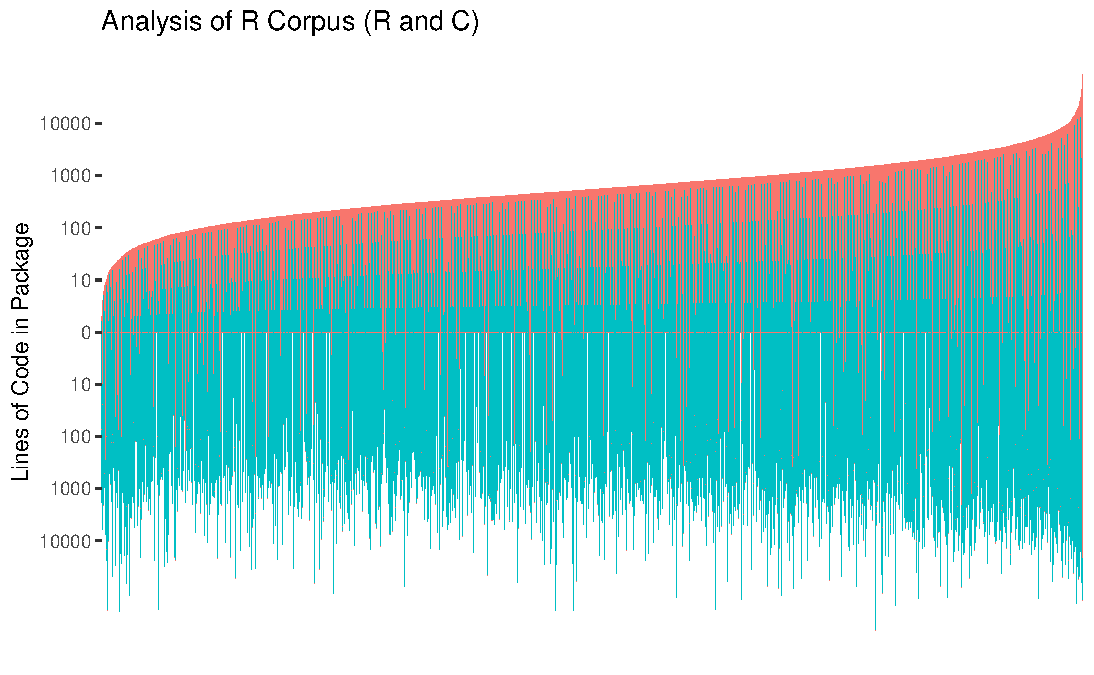
\includegraphics[width=.9\textwidth]{linesofrandccode}
\caption{Lines of code (log scal); for each package, R is above 0, and C/C++
  below}\label{allcloc}\end{center}
\end{figure}


For each package, we extracted all executable code snippets from
documentation, vignettes and tests and ran them independently recording all
calls to R functions.  It is noteworthy that in order to run the scripts in
one package, it is often necessary to load a number of other packages.
In~\cite{issta18}, the authors estimated code coverage to be around 68\%
when including reverse dependencies.  As our infrastructure adds overhead to
script execution, coupled with the fact that some scripts take inordinate
amounts of time to run, this is why we limited our analysis of any given
package to one hour.  

% https://www.r-pkg.org/downloaded
\begin{figure}[!th]{\footnotesize\begin{tabular}{@{}r||l|r|r|r|r|r@{}}\hline
\bf Package & \bf Description & \bf R LOC &\bf C LOC &\bf Scripts & \bf Calls Observed & \bf Calls Recorded \\
\hline
\tt Rcpp  & Seamless C++ integration & 2.2K & 4.2K & 25 & 55K & 340 \\
\tt rlang & Functions for 'Tidyverse' & 7.0K & 6.1K & 122 & 3,924K & 8,422 \\
\tt glue  & Interpreted string literals & 0.3K & 0.3K & 8 & 4K & 145 \\
\tt tibble & Simple data frames & 2.0K & 0.3K & 16 & 1,332K & 6,367 \\
\tt stringi &  String processing & 1.5K & 515K & 64 & 923K & 873 \\
\tt ggplot2 & Data visualisations & 14K & 0 & 130 & 153K & 4,608 \\
\tt dplyr  &  Data manipulation & 4.5K & 4.7K & 78 & 233K & 3,099 \\
\tt pillar & Formatting for columns & 1.4K & 0 & 13 & 803K & 1,514 \\
\tt R6 & Classes w. ref. semantics & 0.7K & 0 & 2 & 1K & 330 \\
\tt stringr & String operations & 0.5K & 0 & 32 & 1,764K & 534 \\
\end{tabular}}\caption{10 Most Downloaded Packages.}\label{most}
\end{figure}

Figure~\ref{most} shows the ten most downloaded CRAN packages.  For each
one, we list how many lines of R and C/C++ the packages contains.  We show
the number of scripts that could be extracted from the package. Each script
corresponds to either one use-case or a set of unit tests. We print the
number of function calls that were observed by our infastructure, and the
number of unique signatures that were recorded.

Our infrastructure only retains unique argument/return combinations. Thus,
while we observe large number of functions being called with different
values, the types of these function call are often similar. Over the entire
corpus, we can see the relation between observed and recorded calls in
Figure~\ref{recorded}.  The median number of observed calls is 82 and
maximum is 19 million.  The median number of recorded signatures is 16 and
the maxium is 8,422. These numbers are skewed by a number of scripts doing
very few calls before plunging into C code.

\begin{figure}[htbp]\begin{center}
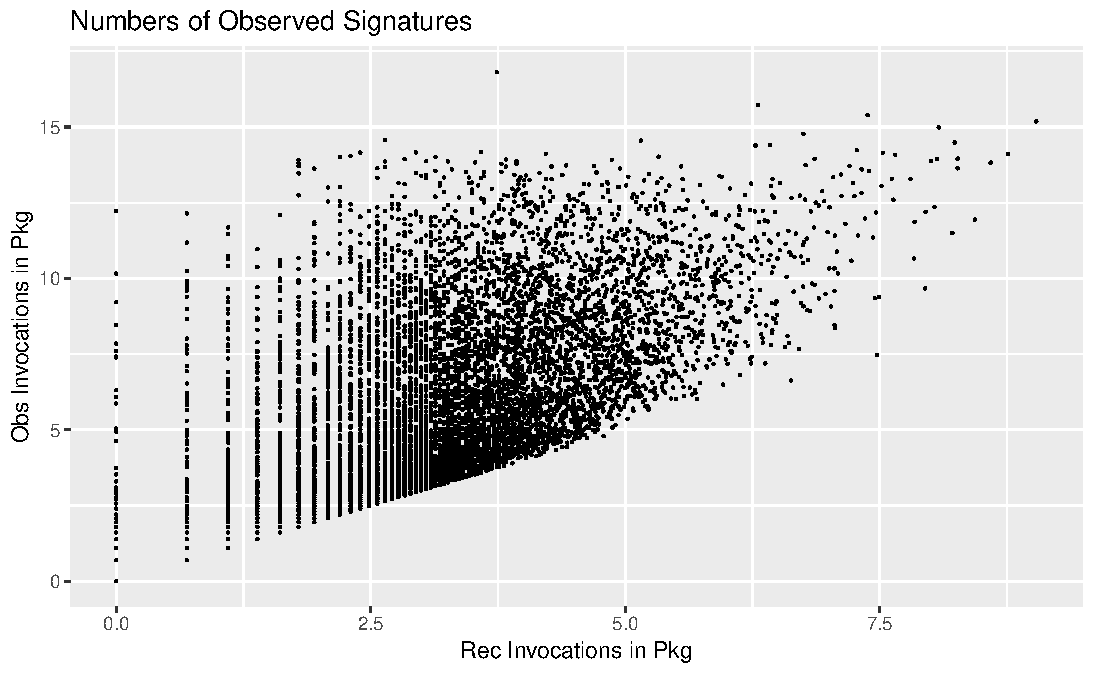
\includegraphics[width=.9\textwidth]{recordsbypkg}
\caption{Numbers of Recorded Function Invocations in the Analyzed Corpus}
\label{recorded}\end{center}
\end{figure}

\newpage
\section{Methods}

In this section, we detail our methodology for collecting data.  Our aim is
to observe arguments and return values of function calls, and from these
generalize possible type signatures for the called functions.  We base our
infrastructure on an open source tool called \genthat whose purpose is to
generate unit tests for R libraries~\cite{issta18}.  \genthat achieves this
by synthesizing unit tests from recorded function argument and return
values, comparing the test against existing ones to avoid generating tests
which do not increase code coverage.  To suit our purposes, we change the
existing tool in two main ways: we record \emph{shapes} rather than values,
and ignore the code coverage optimization phase.  Both changes are
beneficial for scalability, allowing us to trace far more calls.


To illustrate our approach, consider the following script which adds a
double to an integer, and then creates a matrix from a vector, finally
adding them together to get a new matrix.

\begin{figure}[!hb]
\begin{tabular}{ll}\begin{minipage}{5cm}
{\small\begin{lstlisting}[style=R]
> 1 + 2L                     
[1] 3
> x <- c(1,2,3,4)            
> attr(x,"dim") <- c(2,2)    
> x + c(1,2)                 
     [,1] [,2]
[1,]    2    4
[2,]    4    6
\end{lstlisting}}
\end{minipage} & 
\begin{minipage}{8cm}\small
\begin{tabular}{rl}
\tt `+` &\tt D[1], I[1] -> D[1] \\
\tt c& D[1], D[1], D[1], D[1] -> D[4]\\
\tt `<-` &\tt S, D[3] -> D[3]\\
\tt c & \tt D[1], D[1] -> D[2]\\
\tt `attr<-1`&\tt  S, C, D[2] -> \\
\tt c &\tt D[1], D[1] -> D[2]\\
\tt `+` &\tt D[4]{dim=D[2]}, D[2] -> D[4]{dim=D[2]}
\end{tabular}
\end{minipage}
\end{tabular}
\caption{Example script and recorded signature}\label{example}\end{figure}

The functions being called here are \k{`+`}, \k{`<-`}, \k{c} and
\k{`attr<-`}.  The shapes we would expect to record are as follows:
In the above we abreviate types, \k{double}, \k{integer}, \k{symbol} and
\k{character}. For vectorized types we record their length and for all types
we record attributes with some of their values. Looking at the signatures
observed for addition, it is clear that the function is polymorphic as it
starts with the addition of two scalar numbers of different types, and then
adds a matrix to a vector returning a matrix.

\subsection{Implementation}

A high-level description of the workflow of our tool for one package
retrieved from CRAN is as follows:

\begin{enumerate}
\item {\bf Exec generation:} All runnable code in the package is extracted
  from its tests, examples and vignettes. The code snippets are combined
  into a single file.
\item {\bf Installation:} All packages that are required for execution of
  the current package are downloaded and installed.
\item {\bf Instrumentation:} As code is loaded into the R, every function
  definition is instrumented with an \code{on-exit} hook which is invoked
  when the function returns either normally or through an exception.
\item {\bf Recording:} When a hook is called, arguments and return value are
  inspected. We record \k{typeof}, \k{class} and \k{attributes} recursively.
  For \code{list} values, an extra bit of analysis is performed to record
  the element type.
\item {\bf Writing:} Unique signatures are recorded to file with information
  about which package triggered the recording.
\end{enumerate}

Our recording mechanism does not remember the order in which arguments were
passed, nor does it record which arguments were not passed (and for which
default values were used). If an argument was not passed, and no default
value was specified, we record it as \emph{missing}. In R, trying to use
such a missing value results in an error. For practical reasons, we do not
record the contents of environments. These can be used as hash tables and
may be big and are quite likely different from one another.

In R all arguments are passed as promises, and unused arguments will be
unevaluated.  Our tracer does still collect information on these arguments,
as whether or not they were used doesn't change the fact that they were in
fact passed.  In some cases, arguments aren't even intended to be evaluated.
For example, consider the {\tt magrittr} package, which implements the
Tidyverse's pipe functions.  Refer to Figure~\ref{fig:magpipeex} for a
translation of a call to {\tt magrittr}'s pipe ({\tt \%>\%}) function.

\begin{figure}[!hb]{\small\begin{lstlisting}[style=R]
mul_by <- function(x, y) { x * y }

4 %>% mul_by(3) === `%>%`(lhs = 4, rhs = mul_by(3)) === mul_by(4, 3)
\end{lstlisting}}\caption{Example and rough translation of \%$>$\% call.}\label{fig:magpipeex}\end{figure}

Our tracer evaluates function arguments, and here \code{rhs = mul_by(3)},
but that's erroneous code (you can't call {\tt mul\_by} without supplying
two arguments).  In this situation, our tracer will still register the
entire call, but flag the {\tt rhs} argument to indicate to later stages of
the analysis that there was an issue evaluating that argument.

For each function of each package, we consolidate all recorded observations
into a function signature. The details of how consolidation is parameterized
by the definition of a potential type system for R and will be discussed in
the next section.

\section{Stuff}

We will need a notion of polymorphism, and thus a notion of type, when undertaking this analysis. 
R is unityped, and the only notion of polymorphism in the language is its use of dynamic dispatch on the class of an argument.  
For our purposes, we will define a notion in type roughly in line with R's \code{typeof} reflection function, in some cases augmented by information obtained by \code{class} and \code{attributes} reflection.
We start by defining what it means for an {\it argument} to be polymorphic. 

\begin{itemize}
  \item an argument is {\it polymorphic in type} if it has been called with at
  least two distinct types according to our definition of type.
  
   \item an argument is {\it polymorphic in class} if it has been called with at least two distinct classes according to the \code{class} function.
	
  \item attributes are a bit more tricky.  We can't simply count the number of
  attributes that have inhabited an argument, since values can contain
  arbitrarily many attributes (and having several attributes isn't
  polymorphism---think records).  Instead, we define the {\it attribute
    pattern} of a value to be the set of all attribute name and type pairs
  in the attribute list of a value (obtained via \code{attributes}).  And so
  an argument is {\it polymorphic in attribute} if it has been called with
  at least two distinct attribute patterns.

\end{itemize}

The main ingredient of our types is the {\tt typeof} a value, and there is an important distinction to be made between the result of \code{typeof} and that of \code{class} and \code{attributes}.
In R, the \code{typeof} a value cannot change, and this is not the case with class and attributes.  
As mentioned in \AT{an earlier section}, the class of values can be easily redefined by assigning to the value's class attribute, and similarly attributes can be dynamically added, removed, or changed.

While we do consider some class and attribute information when constructing our types, it is also valuable to consider them entirely separate from types.
Users are free to define their own classes, and arbitrarily add and remove attributes, and interesting patterns might arise in considering them.
That said, not attribute patterns and classes are necessarily interesting, and indeed some of R's built-in data structures use them to some extend.
For one, data frames have a {\tt data.frame} class (explicitly on the class attribute).
Other standard patterns are:

\begin{itemize}

\item data frames have three attributes: {\tt names} for column names, {\tt
  row.names} for row names, and {\tt class} (which is instantiated to {\tt
  "data.frame"} upon creation).
	
\item matrices have at least a {\tt dim} attribute with matrix dimensions,
  and optionally a {\tt dimnames} attribute for dimension names. Curiously, the {\tt dim} attribute is all that is needed to define a matrix (i.e., a list with a {\tt dim} attribute {\it is} a matrix).

\item lists and vectors may have a {\tt names} attribute, which assigns
  names to locations.
	
\item to ease dealing with large sorted sets of non-numeric values, R offers
  the \code{factor} and \code{levels} functions.  \code{factor(x,
    levels=someOrder)} adds a {\tt "levels"} attribute to \code{x}, which
  specifies an ordering for \code{x} according to the \code{sortedOrder}
  parameter.  \code{factor} also changes the class of the parameter being
  factored to \texttt{"factor"}.

\end{itemize}

These naturally-occurring attribute patterns and classes can be separately
accounted for to highlight user-defined patterns and behaviors.  This will
be made clear in Section~\ref{sec:results}.

%
%
%
%
\subsection{Granularity of Type Information}

When constructing a type for a value, we begin with the {\tt typeof} the value.
This alone paints an incomplete picture of the value, though, especially when it comes to vectors (recall that \code{typeof(5) == typeof(c(5, 5)) == "double"}).
In some cases, the class or attributes of a value might enlighten us, but in many cases we can be a little more precise.

To be as specific as possible, our analysis collects additional information
to create a more specific type than the result of any of R's reflection
functions.  The details of the information we collect follows.

\begin{itemize}

	\item if the analysis encounters \code{ typeof(x) == "double"}, it will look at the length of {\tt x} to determine if {\tt x} is a scalar or a vector, generating the annotation {\tt scalar/double} or {\tt vector/double} accordingly.
	This is also true for integer, complex, raw, logical, and character {\tt typeof}s (i.e., the primitive vectorized data types).
	A notable imperfection here is is that unit length vectors will appear as scalars, so later in our analysis we ensure that argument signatures containing both scalar/X and vector/X are collapsed down to contain only vector/X.
	
	\item if the analysis encounters \code{typeof(x) == "list"}, we collect type information on all list elements in order to ascribe a general type to the contents of the list.
	To avoid undue slowdowns, we only collect the \code{typeof} the contents, and ascribe type {\tt any} if two or more {\tt typeof}s are observed.
	
	\item if the analysis encounters \code{NA}, we ascribe a unique {\tt raw\_NA} type.
	In R, \code{NA} inhabits all types, but \code{typeof(NA) == "logical"}.
	The analysis deals with these {\tt raw\_NA}s at a later stage.
	
	\item if the analysis encounters a matrix (i.e. the value has matrix class and has a dims and optionally dimnames attribute), we ascribe the type {\tt matrix}.
	
	\item similarly, if it encounters a data frame (i.e., class {\tt data.frame} with appropriate attributes), we ascribe the type {\tt data.frame}.

\end{itemize}

%
%
%
%
%
%
\section{Examples of Polymorphism}
\label{sec:polyex}

\AT{Putting examples of polymorphism in this section, we can talk about them and where they should go.}

First, Figure~\ref{fig:realex} shows an example of how integers and doubles are very compatible.
\AT{TODO add matrix (dimensions) to the example.}

\begin{figure}[!hb]{\small\begin{lstlisting}[style=R]
> 5L + 1L # => 6L, an integer
> 5L + 1.2 # => 6.2, a double (5L coerced to 5.0)
> c(10, 20, 30)[1.2] # => 10, 1.2 coerced to 1L
\end{lstlisting}}\caption{Example of {\it real} type usage.}\label{fig:realex}\end{figure}

Figure~\ref{fig:optnull} shows an example of a function with an optional argument.
In the function, {\tt x} is a sorted vector of income values, and {\tt w} is a vector of weights, optionally NULL.
The function computes fractional ranks required for the computation of some coefficient implemented by the package.
We see that if {\tt w} is NULL, then default unit weights are generated.

\begin{figure}[!hb]{\small\begin{lstlisting}[style=R]
frac.ranks <- function(x, w=NULL) {
  if (is.null(w)) w <- rep(1, length(x)) # if no weights passed, take all weights = 1
  ...
\end{lstlisting}}\caption{Example of optional argument (from {\tt acid} package).}\label{fig:optnull}\end{figure}

Figure~\ref{fig:listvec} shows an example of a function with list and vector polymorphism.
The function takes a list or vector {\tt point} and a data frame {\tt polyg} representing a polygon.
In it, we see that {\tt point} can be either a list or a vector, and the function code casts the argument to a double vector.

\begin{figure}[!hb]{\small\begin{lstlisting}[style=R]
is.point.inside <- function (point, polyg) {
    p <- as.numeric(point) # as.numeric(list(1, 2)) => c(1, 2)
    ...
\end{lstlisting}}\caption{Example of list/vector argument (from {\tt bivrp} package).}\label{fig:listvec}\end{figure}

Figure~\ref{fig:charclos} shows an example of a function with character and function polymorphism.
\AT{Bluh.}
At a high level, this function calculates point estimates for an {\tt angmcmc} object (specific to some packages).
The caller specifies {\tt fn}, either a function or a function name which will be evaluated on the object samples to estimate parameters.
The call to lookup the function name is on line 10.

\begin{figure}[!hb]{\small\begin{lstlisting}[style=R]
pointest <- function (object, fn = mean, par.name, comp.label, chain.no,  ...) {
    ...
    if (is.character(fn)) {
        if (fn == "MODE" | fn == "MAP") {
            do_MAP <- TRUE
        }
        else {
            do_MAP <- FALSE
            fn <- match.fun(fn) # looks up the function name
        }
    }
    ...
\end{lstlisting}}\caption{Example of char/closure argument (from {\tt BAMBI} package).}\label{fig:charclos}\end{figure}

\AT{I'll explain this better, maybe?}
In Figure~\ref{fig:dfdbl}, we see a function that, among other things, takes in some data ({\tt dat}) and a character string ({\tt spss}) specifying either {\tt "in"} or {\tt "out"}.
Now, depending on the value of {\tt spss}, {\tt dat} will either be a data frame or a vector of doubles.

\begin{figure}[!hb]{\small\begin{lstlisting}[style=R]
nret.translator <- function(dat, spss="out", ...) {
  ...
  if(identical(spss, "out")) {
    if(!is.vector(dat)) {
        stop(simpleError("...'dat' must be a vector!"))
      }
    ...
  } else {
    ...
    # here, dat is data.frame
    items.idx <- items.idx[order(names(dat[, items.idx]))]
  }
\end{lstlisting}}\caption{Example of a data.frame/(vector/double) argument (from {\tt klausR} package).}\label{fig:dfdbl}\end{figure}

In Figure~\ref{fig:chardbl}, we see a function which takes in a list ({\tt network}), a vector of indices of that list ({\tt fixIndices}), and a vector of values ({\tt values}).
The locations specified by {\tt fixIndicies} in {\tt network} are updated with {\tt values}.
Here, {\tt fixIndicies} has been observed to be either a character or double vector:
In R, list indices are typically doubles, but can be characters (if the list or vector being indexed has a {\tt names} attribute).

\begin{figure}[!hb]{\small\begin{lstlisting}[style=R]
fixGenes <- function (network, fixIndices, values) {
  ...
  network$fixed[fixIndices] <- as.integer(values)
  ...
}
\end{lstlisting}}\caption{Example of character/double argument (from {\tt BoolNet} package).}\label{fig:chardbl}\end{figure}

In Figure~\ref{fig:matvec}, we see that the function can take in a vector, but immediately transforms it (transpose, with {\tt t}) into a matrix.
As an idea, matrix/vector polymorphism seems sensible, as mathematically vectors are matrices.
R echoes this by making conversion between the two ``types'' easy:
\code{as.vector(m)} flattens a matrix \code{m} into a vector (e.g., \code{as.vector(matrix(2, 2, 2)) == c(2, 2, 2, 2)}), and \code{as.matrix(v)} builds a {\tt length(v) x 1} matrix (e.g., \code{as.matrix(c(1, 2)) == matrix(data=c(1, 2))}).
\AT{TODO fix line break in code at end of last sentence}

\begin{figure}[!hb]{\small\begin{lstlisting}[style=R]
tee <- function (x, theta, D1, D2, phi)  {
    if (is.vector(x)) {
        x <- t(x)
    }
    ...
\end{lstlisting}}\caption{Example of matrix/(vector/double) argument (from {\tt calibrator} package).}\label{fig:matvec}\end{figure}

%
%
%
%
%
%
\section{Results}\label{sec:results}

Having built an understanding of our data collection and analysis pipeline, we will turn our attention to the results of our analysis.  

\AT{Maybe it's best to ignore attributes and classes for now?}

%
%
%
%
\subsection{L0}

The logical ``baseline'' for the design of a static type system for R is promotion of the language's dynamic types (in the sense of \code{typeof}) to static types; we call this type system L0.
Such a type system exactly reflects the types of values in the R runtime environment, as the \code{typeof} an object is in direct correspondence with the runtime type tag of the value.

In this section, we will begin by breaking down our corpus of data with L0 in mind.
From this perspective, we will see how current R programmers see types in the language, and we will leverage our newfound insight to design a type system which should be relevant to them.

Without further ado, let's look at the data, first focusing on a broad overview of the polymorphism in L0.
Figure~\ref{fig:L1argcounts} shows the polymorphicity of argument positions in R function.
From there, we build up a picture of the polymorphicity of functions as a whole, and the data for this function polymorphism can be found in Figure~\ref{fig:L1funcounts}.

% latex table generated in R 3.5.1 by xtable 1.8-3 package
% Fri Mar 29 18:10:23 2019
\begin{table}[ht]
\label{fig:L1argcounts}
\centering
\begin{tabular}{lrr}
  \hline
Type & Count & Percentage \\ 
  \hline
Full Monomorphic & 784K & 85.76 \\ 
  Monomorphic in Type & 845K & 92.46 \\ 
  Monomorphic in Class & 827K & 90.41 \\ 
  Monomorphic in Attribute Pattern & 825K & 90.27 \\ 
  Total Seen & 914K & --- \\ 
   \hline
\end{tabular}
\caption{typeof type system (L0) (arguments)}
\end{table}
% latex table generated in R 3.5.1 by xtable 1.8-3 package
% Fri Mar 29 18:10:23 2019
\begin{table}[ht]
\label{fig:L1funcounts}
\centering
\begin{tabular}{lrr}
  \hline
Type & Count & Percentage \\ 
  \hline
Full Monomorphic & 144K & 66.54 \\ 
  Monomorphic in Type & 173K & 80.16 \\ 
  Monomorphic in Class & 163K & 75.21 \\ 
  Monomorphic in Attribute Pattern & 161K & 74.37 \\ 
  Total Seen & 216K & --- \\ 
   \hline
\end{tabular}
\caption{typeof type system (L0) (functions)}
\end{table}

From Figure~\ref{fig:L1argcounts}, we glean that argument positions aren't very polymorphic in L0.
An argument which is "Monomorphic in Type" is monomorphic w.r.t. \code{typeof}, in that it was only ever observed to have one \code{typeof}.
Similarly, an argument is "Monomorphic in Class" if it is only ever called with one {\tt class}.
As we said earlier, attributes are a little more complicated, and an argument which is "Monomorphic in Attribute Pattern" was only ever observed to have one attribute pattern (and that pattern may itself contain many attributes).

As for the polymorphism of functions as a whole, we glean from Figure~\ref{fig:L1funcounts} that a sizeable number of functions are polymorphic.
Functions are said to be polymorphic if at least one of their arguments or return are polymorphic.
\AT{Say more?}

At present, we will only concern ourselves with \code{typeof} polymorphism, and we will later worry about classes and attributes.
To get an idea of what kinds of polymorphism occur, we will look at the most commonly occurring polymorphic argument signatures.
Table~\ref{tab:L1toppoly} has the top polymorphic signatures for L0.

% latex table generated in R 3.5.1 by xtable 1.8-3 package
% Fri Mar 29 18:13:17 2019
\begin{table}[ht]
\label{tab:L1toppoly}
\centering
\begin{tabular}{lrr}
  \hline
type & count & perc \\ 
  \hline
  double, integer & 19,799 & 28.73 \\ 
  double, list & 5,324 & 7.72 \\ 
  double, NULL & 5,152 & 7.48 \\ 
  character, NULL & 3,682 & 5.34 \\ 
  double, logical & 3,388 & 4.92 \\ 
  character, double & 2,842 & 4.12 \\ 
  list, NULL & 2,799 & 4.06 \\ 
  character, list & 1,836 & 2.66 \\ 
  character, integer & 1,663 & 2.41 \\ 
  character, double, integer & 1,362 & 1.98 \\ 
   \hline
\end{tabular}
\caption{Top polymorphic signatures for the L0 type system.}
\end{table}

Some entries in the Table~\ref{tab:L1toppoly} are clear (e.g., double, integer polymorphism is unsurprising), others are strange (e.g., character, double), but in fact they all have some explanation.

\begin{enumerate}

	\item \{double, integer\}: in R, doubles and integers are effectively interchangeable, as casting from one to the other is straightforward and automatically performed when appropriate.
	For example, \code{c(1, 2)[1.9] == 1}.
	This distinction is mainly just relevant to the implementation, as integers and doubles are stored and dealt with differently in the runtime but programmers only see the distinction when printing.
	
	\item \{double, list\} and \{character, list\}: at first glance, these type signatures are suspect.
	Why would so many programmers want to pass a double or a list to some function?
	The key insight here is that doubles and characters are {\it vectorized} in R, meaning that a double is really a vector of doubles.
	Thus, these seemingly strange signatures are revealed to be entirely reasonable: these signatures are likely to describe arguments which are either vectors or lists.
	
	\item \{X, NULL\}: in most languages, NULL is an inhabitant of all types, and we see that this is not the case in R.
	That said, there is a pattern of many functions having default or optional arguments, and in many of these cases NULL is the default value.
	
	\item \{double, logical\}: the first values of type logical that come to mind are TRUE and FALSE, which does little to explain this strange signature.
	Indeed, the key here is an implementation detail of R's: recall that NAs inhabit every type.
	As it happens, the default type of NA is logical (e.g., \code{typeof(NA) == "logical"}), and this is likely what is being seen here.
	We will control for this by distinguishing NAs with their own type, {\tt raw\_NA}, but we will get to that in time.
	
	\item \{character, double\}, \{character, integer\} and \{character, double, integer\}: yet more strange signatures.
	These signatures are a little more subtle to explain.
	For one, indexing lists and vectors can be done with either strings (i.e., to access a named index) or with numbers.
	Another option is dates: R has many ways to present dates, and strings and numbers feature among them.
	Finally, many \AT{get numbers} functions in R return a string if an error occurs during execution.

\end{enumerate}

How will we deal with this?

\begin{enumerate}

	\item consolidating doubles and integers into a single real-number type would account for all of this polymorphism.
	
	\item to get an idea of how often vectors and lists co-occur in signatures, we need to expand our analysis of vectorized types.
	Notably, when we encounter e.g. a double, we should collect length information to see if the double is a vector of doubles or just a scalar.
	This will feature in our next type system, L1, which we will get to momentarily.
	
	\item if we roll NULLs into every type, we can cleanly deal with these X, NULL signatures.
	As we have established that an annotation for an optional argument is useful, this will allow us to reveal other interesting patterns.
	\AT{If we feel the need to go into more details on NULL or NA, I have the old paragraphs commented out in the source.}
	
	\item similarly with NULLs, we're interested in rolling NAs in to all types.
	As we mentioned, this is actually what the R runtime does, but a default type needed to be chosen for NAs appearing without context.
	Subsuming NAs should help to reveal other interesting patterns.
		
	\item dealing with this polymorphism will be more tricky.
	We might need to pull class information in (to pick up on dates), and possibly make a signature judgment depending on which argument position has the signature (e.g. a \{character, X\} signature on a return).
	We will come back to this later.

\end{enumerate}

There are some clear limitations to the L0 type system that we should address before working through any of these other issues
As we mentioned, \code{typeof} makes no distinction between vectors and scalars, as indeed there is no such distinction in R. 
But as we saw, we might benefit from such a distinction, and indeed an all-new runtime environment design for R might benefit from e.g. not needing to vectorize scalar values.
This is one of the many modifications we make, all of which are thoroughly explored in the following section.

%In terms of programmer behavior, we observe a pattern of optional arguments throughout several R packages, wherein programmers specify a default argument value which is sometimes NULL.
%Consider the snippet in Figure~\ref{fig:optnull} for an example.
%\AT{TODO put that figure here}
%The distinction between NULL and other types is not particularly useful to the programmer, so we propose to also collapse this distinction.
%Not pictured in Table~\ref{tab:toppolyFDTS} are NAs, which are ascribed the type {\tt raw\_NA} in L1; NAs in fact inhabit every type, though the default NA type is {\tt logical}.
%Just as we fold NULL into all types, we will do the same with NAs.

%
%
%
%
\subsection{L1}

To address these limitations, we augment the L0 with more fine-grained information.
We will consider unit-length vectors to be scalars, collect list member type information to build an accurate list type, and promote NAs to their own type. 
In addition, we collect attribute and class information to distinguish a type for data frames and matrices, as the \code{typeof} these is simply {\tt list} in R. 
We refer to this as the L1 type system. 
An example of a signature in this type system can be found in Figure~\ref{fig:exL1}.

\begin{figure}[!hb]{\small\begin{lstlisting}[style=R]
add_make_list <- function(x, y) {
  l <- as.list(x + y)
  attr(l, "example") <- "this is an attribute"
  l
}
add_make_list(2, c(3, 1)) # => list(5, 3)
\end{lstlisting}}

\begin{tabular}{@{}r|l|l|l@{}}\hline
\bf Argument & \bf Type & \bf Class &\bf Attributes \\
x & \tt scalar/double & \tt numeric & \tt \{\} \\
y & \tt vector/double & \tt numeric & \tt \{\} \\
retv & \tt list<double> & \tt list & \tt \{example: scalar/character\}  
\end{tabular}
\caption{Example call and L1 signature.}\label{fig:exL1}\end{figure}

Let us begin as we did in L0 by looking at the amount of polymorphism in L1.
The data can be found in Tables~\ref{tab:argcountsL1}~and~\ref{tab:funcountsL1}.
\AT{TODO: have these tables be generated automatically}

% latex table generated in R 3.5.1 by xtable 1.8-3 package
% Fri Mar 22 18:03:30 2019
\begin{table}[ht]
\label{tab:argcountsL1}
\centering
\begin{tabular}{lrr}
  \hline
 Argument Polymorphism & Count & Percentage \\ 
  \hline
  Full Monomorphic & 781K & 85.37 \\ 
  Monomorphic in Type & 834K & 91.23 \\ 
%  Monomorphic in Class & 827K & 90.42 \\ 
%  Monomorphic in Attribute Pattern & 825K & 90.27 \\ 
  Total Seen & 914K & --- \\ 
     \hline
\end{tabular}
\caption{Account of {\it argument} polymorphism in L1.}
\end{table}

% latex table generated in R 3.5.1 by xtable 1.8-3 package
% Fri Mar 22 18:10:46 2019
\begin{table}[ht]
\label{tab:funcountsL1}
\centering
\begin{tabular}{lrr}
  \hline
 Function Polymorphism & Count & Percentage \\ 
  \hline
  Full Monomorphic & 143K & 65.88 \\ 
  Monomorphic in Type & 167K & 77.25 \\ 
%  Monomorphic in Class & 163K & 75.24 \\ 
%  Monomorphic in Attribute Pattern & 161K & 74.37 \\ 
  Total Seen & 216K & --- \\ 
   \hline
\end{tabular}
\caption{Account of {\it function} polymorphism in L1.}
\end{table}

\AT{We should figure out the pipeline to get the notebook output into here automatically.}

We see that roughly 9\% of all argument positions in L1 are polymorphic in type, as opposed to 7.5\% in L0.
This small difference is perhaps surprising, as we did define a number of additional types and might expect for there to be a lot more polymorphism.
This is explained by the fact that drawing the distinctions added a lot of polymorphism to already polymorphic arguments.
\AT{We can get numbers on this.}

As for functions, roughly 23\% are polymorphic in type, or put differently 23\% have at least one polymorphic argument or a polymorphic return.
Again, the small difference between L0 and L1 in this regard is explained by a tendency to make already polymorphic functions more polymorphic.

As before, these numbers alone are insufficient, so we ask again: {\it of the polymorphic arguments, what are the most common patterns?}
The answer to that question can be found in Table~\ref{tab:toppolyL1}.

% latex table generated in R 3.5.1 by xtable 1.8-3 package
% Fri Mar 22 21:27:37 2019
\begin{table}[ht]
\label{tab:toppolyL1}
\centering
\begin{tabular}{lrr}
  \hline
 Polymorphic Type Signature & \# Occurrences & \% of Total Polymorphism \\ 
  \hline
  vector/double, vector/integer & 7742 & 9.66 \\ 
  scalar/double, scalar/integer & 7201 & 8.99 \\ 
  matrix, vector/double & 5384 & 6.72 \\ 
  NULL, scalar/character & 2325 & 2.90 \\ 
  list$<$any$>$, list$<$double$>$ & 2231 & 2.78 \\ 
  data.frame, matrix & 2116 & 2.64 \\ 
  NULL, scalar/double & 2082 & 2.60 \\ 
  NULL, vector/double & 2069 & 2.58 \\ 
  list$<$any$>$, list$<$list$>$ & 1432 & 1.79 \\ 
  NULL, vector/character & 1380 & 1.72 \\
     \hline
\end{tabular}
\caption{Top polymorphic argument signatures in the L1.}
\end{table}

We would like to make one important note before digesting the data in Table~\ref{tab:toppolyL1}.
We drew a distinction between scalars and vectors of the same type, and that distinction would be the single largest source of polymorphism in L1 had we not dealt with it appropriately.
We note that an argument which exhibits a signature including e.g. \{scalar/double, vector/double\} really must be an argument designed to take vectors, as recall that unit length vectors appear as scalars by our definition.
We have already collapsed this distinction.

In Table~\ref{tab:toppolyL1}, we again see the prominence of {\tt double} and {\tt integer} polymorphism.
As discussed previously, we will address this by creating a new {\it real} type encompassing both.
Refer back to the snippet in Figure~\ref{fig:realex} for details.
Also, another clear pattern in Table~\ref{tab:toppolyL1} is that of NULL, X.
As we discussed, we will roll NULL (and raw NAs) into other types.

%
%
\subsubsection{Scalars}

As we make the distinction between vectors and scalars, one other interesting question that arises is: {\it how many arguments are strictly scalar?}
As it happens, over 40\% of monomorphic arguments with primitive vectorized types are always scalar (so, 40\% of {\it monomorphic} occurrences of {\tt scalar/X} and {\tt vector/X} are scalar).
This shows that there is value in a scalar annotation, which could be used to communicate to an R runtime that vectorization of a value is not necessary, which may in turn lead to a performance improvement.

At this point, we have seen a number of reasonable polymorphic patterns that arise in R, both in L0 and L1.
The next type system design we consider will deal with these, and we refer to it as L$1^{+}$.
The number of monomorphic arguments and functions can be found in Tables~\ref{tab:argcountsL1p} and~\ref{tab:funcountsL1p} respectively.

% latex table generated in R 3.5.1 by xtable 1.8-3 package
% Fri Mar 22 18:03:30 2019
\begin{table}[ht]
\label{tab:argcountsL1p}
\centering
\begin{tabular}{lrr}
  \hline
 Argument Polymorphism & Count & Percentage \\ 
  \hline
  Full Monomorphic & 781K & 85.47 \\
  Monomorphic in Type & 867K & 95.01 \\
%  Monomorphic in Class & 831K & 90.31 \\ 
%  Monomorphic in Attribute Pattern & 830K & 90.25 \\ 
  Total Seen & 914K & --- \\ 
     \hline
\end{tabular}
\caption{Account of {\it argument} polymorphism in L$1^{+}$.}
\end{table}

% latex table generated in R 3.5.1 by xtable 1.8-3 package
% Fri Mar 22 18:10:46 2019
\begin{table}[ht]
\label{tab:funcountsL1p}
\centering
\begin{tabular}{lrr}
  \hline
 Function Polymorphism & Count & Percentage \\ 
  \hline
  Full Monomorphic & 143K & 66.04 \\ 
  Monomorphic in Type & 184K & 85.30 \\
%  Monomorphic in Class & 163K & 75.13 \\ 
%  Monomorphic in Attribute Pattern & 161K & 74.31 \\ 
  Total Seen & 216K & --- \\ 
   \hline
\end{tabular}
\caption{Account of {\it function} polymorphism in L$1^{+}$.}
\end{table}

We had some big wins here, with only ~5\% of argument polymorphism unaccounted for.
To get an idea of what more we can do, let's see what the most frequent remaining polymorphic signatures are.
See Table~\ref{tab:toppolyL1p}.

% latex table generated in R 3.5.1 by xtable 1.8-3 package
% Tue Mar 26 17:46:45 2019
\begin{table}[ht]
\label{tab:toppolyL1p}
\centering
\begin{tabular}{lrr}
  \hline
Polymorphic Type Signature & \# Occurrences & \% of Total Polymorphism \\ 
  \hline
  matrix, vector/real & 6360 & 13.94 \\ 
  list$<$any$>$, list$<$real$>$ & 2799 & 6.13 \\ 
  vector/character, vector/real & 2774 & 6.08 \\ 
  scalar/character, scalar/real & 2552 & 5.59 \\ 
  data.frame, matrix & 2167 & 4.75 \\ 
  list$<$any$>$, list$<$list$>$ & 1496 & 3.28 \\ 
  list$<$any$>$, list$<$character$>$ & 1214 & 2.66 \\ 
  data.frame, vector/real & 1046 & 2.29 \\ 
  scalar/logical, scalar/real & 920 & 2.02 \\ 
  scalar/character, vector/real & 868 & 1.90 \\
   \hline
\end{tabular}
\caption{Top 10 argument signatures in L$1^{+}$.}
\end{table}

A few of the top polymorphic signatures stand out.
First, the matrix/(vector/real) signature is interesting: \AT{as we showed in our polymorphism examples section}, converting between vectors and matrices is very simple, and indeed numeric vectors are mathematically {\tt 1 x n} matrices.
In fact, in R matrices can be used identically to vectors in many cases, and we refer the reader to Figure~\ref{fig:matasvec} for examples.
\begin{figure}[!hb]{\small\begin{lstlisting}[style=R]
v <- c(1, 2, 3, 4)
ma <- matrix(data=v, nrow=4, ncol=1)
v[2] == m[2] == m[2, 1]

mb <- matrix(data=v, nrow=2, ncol=2)
v[3] == m[3] == m[1, 2] 
\end{lstlisting}}\caption{Using a matrix like a vector.}\label{fig:matasvec}\end{figure}

\AT{We should figure out how we want to deal with this polymorphism.}

\AT{list<list> might be objects?}

Another significant source of apparently strange polymorphism is the {\tt character}, {\tt real} polymorphism.
Recall Figure~\ref{fig:chardbl}, which laid out an example of this polymorphic signature: lists and vectors can be accessed by strings as well as by numerics.
This is a somewhat unusual example of polymorphism, and our argument depends on there being perhaps a list or vector passed alongside the {\tt character}- or {\tt real}-typed argument.
So, just how often is this the case?
Well, as it happens, character/real polymorphism coincides with some list-flavored type in \INDEXCOINCIDENCE instances (\INDEXYPERC of occurrences).

Another option is a date.
In R, dates are often represented as either strings or numbers, and many packages make use of dates.
Dates (sometimes) manifest themselves in the {\tt class} of a value, for examples refer to Figure~\ref{fig:date}.
\begin{figure}[!hb]{\small\begin{lstlisting}[style=R]
class(date()) # => character
class(Sys.Date()) # => Date
class(as.POSIXlt(Sys.Date())) # => POSIXlt, POSIXt
as.integer(as.Date(1, origin = "1900-01-01"))
\end{lstlisting}}\caption{Dates in R.}\label{fig:date}\end{figure}

This figure reveals an unfortunate truth that date ``data type'' in R is not standardized.
That said, translating between the data types is straightforward.

We have seen that once we have done away with trivial sources of polymorphism, a number of interesting patterns arise.
In many of these cases, we can appeal to other sources of reflection in R to expand our understanding.
For example, to deal with the possibility of dates, we can appeal to the \code{class} of values, and to gain more information on matrices we might be interested in looking at attributes.
The next type system addresses these concerns.

%
%
%
%
\subsection{L2}

\AT{Eyy time for L2.}

%
%
%
%
\AT{We might want to discuss some of the most polymorphic functions in the language.}
\subsection{R's Most Polymorphic Functions}

In this section, our goal is to shed some light on the most polymorphic functions in R.
Table~\ref{tab:bigpolyfuns} shows the 10 functions with the biggest recorded signatures.

% latex table generated in R 3.5.1 by xtable 1.8-3 package
% Thu Mar 28 16:01:37 2019
\begin{table}[ht]
\label{tab:bigpolyfuns}
\centering
\begin{tabular}{llrl}
  \hline
Package & Function & Size & Description \\ 
  \hline
magrittr & \%$>$\% & 23.00 & Tidyverse pipe function \\ 
  magrittr & freduce & 17.67 & Apply a list of functions sequentially \\ 
  rlang & captureArgInfo & 16.50 & Capture arg info \\ 
  rlang & enquo & 16.00 & Create quosure \\ 
  rlang & get\_expr & 15.00 & Extract expression \\ 
  data.table & replace\_dot\_alias & 13.50 & Deals with '.' in passed expr \\ 
  tibble & strip\_dim & 13.00 & Removes 'dim' attribute \\ 
  data.table & copy & 11.00 & Create copy of passed value \\ 
  htmlwidgets & shouldEval & 11.00 & Eval passed value depending on tag \\ 
  magrittr & \%$<$$>$\% & 11.00 & Like \%$>$\% but assigns \\ 
   \hline
\end{tabular}
\caption{10 most polymorphic functions.}
\end{table}

The size metric we use is roughly the size of each individual argument signature, divided by the number of function arguments.
The division is performed to avoid unfairly favouring functions with many arguments.

Which packages are the most polymorphic?
Figure~\ref{tab:packagepolysize} has the answer.

% latex table generated in R 3.5.1 by xtable 1.8-3 package
% Thu Mar 28 18:15:26 2019
\begin{table}[ht]
\label{tab:packagepolysize}
\centering
\begin{tabular}{lrl}
  \hline
Package & Total Size & Description \\ 
  \hline
  magrittr & 4.16 & Tidyverse pipe suite \\ 
  types & 3.25 & Simple type annotations for R \\ 
  r6extended & 3.00 & Utilities extending barebones R6 package \\ 
  utils & 2.93 & Utilities for R developers \\ 
  zeallot & 2.85 & Metaprogramming package for assignment \\ 
  listviewer & 2.72 & R list visualizer \\ 
  proto & 2.60 & Prototype object-based programming \\ 
  apercu & 2.49 & Display a short view of a complex R value (list, vector, etc.) \\ 
  pipeR & 2.46 & Another pipe suite \\ 
  rethinker & 2.44 & RethinkDB client for R \\ 
   \hline
\end{tabular}
\caption{10 most polymorphic packages.}
\end{table}

\AT{Draft}



The most polymorphic function in the corpus of code we analyzed is {\tt magrittr}'s {\tt \%>\%} (pipe) function.
{\tt magrittr} is part of the Tidyverse, and the pipe function is frequently used to chain function calls.
The fact that the pipe is the most polymorphic function is not shocking, as its goal is simply to take the right hand argument and apply it to the left hand argument, and this in a sense irrespective of type.

...

%
%
%
%
\subsection{Metaprogramming}

\AT{Will probably change.}

Tidyverse owes some of its success to the new syntax defined by some of the included packages.
One such example is the pipe operator \%$>$\% that we saw in the last section, and indeed this function was highly exercised by many other packages \AT{get counts}.
We also grappled with the unfortunate truth that arguments to \%$>$\% can't always be evaluated, which causes some annoyances in the analysis.

We would like to know how often packages contain functions designed for metaprogramming.
As it happens, when arguments fail to evaluate during our analysis even as functions execute successfully, we are actually dealing with instances of metaprogramming.
Some functions, such as those in the magrittr package, will take one (or more) of their arguments and use them as an AST, performing surgery on the expression to create some new expression that they evaluate.
Sometimes, these arguments intended for metaprogramming {\it will} successfully evaluate in our tracer, but this is merely chance.
For example, consider the code snippet in Figure~\ref{fig:metaexworks}.

\begin{figure}[!hb]{\small\begin{lstlisting}[style=R]
mul_by_w_defaults <- function(x=1, y=1) x * y

4 %>% mul_by_w_defaults(2) == `%>%`(lhs = 4, rhs = mul_by(3)) 
\end{lstlisting}}\caption{Dates in R.}\label{fig:metaexworks}\end{figure}

In this example, our analysis will successfully evaluate the {\tt rhs} argument 

%
%
%
%
\subsection{Function Polymorphism}

Now, we will turn our attention to whole function polymorphism.

This is different because we can now look at argument polymorphism across several arguments, like we did when thinking about character/real polymorphism.

We're interested to see what kinds of ``meta-annotations'' we can make at the function level.
For instance, should we link argument types with return types?
Consider Figure~\ref{fig:funanno}.
\begin{figure}[!hb]{\small\begin{lstlisting}[style=R]
iden <- function(x) x;

# observed calls:
f(2); # x: double -> double
f(list(1, 2, 3)) # x: list<double> -> list<double>

# possible annotations:
# [1] x: {double, list<double>} -> {double, list<double>}
# [2] x: {double -> double, x: list<double> -> list<double>}
\end{lstlisting}}\caption{Possible function annotations.}\label{fig:funanno}\end{figure}
\AT{Say more about this?}

Harkening back to our discussion of character/real polymorphism, we mentioned that we might want to consider such a type signature to be a list or vector index only if a list or vector was present as another argument.
Now, this may be moving well beyond the purview of R programmers, but perhaps there is value in such a scenario, particularly if we include even {\it more} information in a type system.
For example, say we have a function which takes in a 2D point list.
There are a plethora of useful annotations, here, and of varying degrees of granularity.
We might want simply a "list" annotation, or we might want a "list<double>" annotation to be more specific.
In addition, though, we might want to know if the list has a names attribute, yielding "list<double>@names".
Then, perhaps it would be useful to know what the names were, so "list<double>@names\{x, y\}".

Now, depending on the granularity of individual argument annotations, we might want to link certain arguments together.
Consider the code snippet in Figure~\ref{fig:indexof}.
\begin{figure}[!hb]{\small\begin{lstlisting}[style=R]
access <- function(l, i) l[[i]]

L <- list(a=1, b=2, c=3)
access(L, 2) # => 2
access(L, "c") # => 3

# possible annotations:
# [1] l: list, i: {character, real} -> real
# [2] l: list<double>, i: {character, real} -> real
# [3] l: list<X>, i: {character, real} -> X
# [4] l: list<double>@names, i: index -> double
# [5] l: list<double>@names{a, b, c}, i: index@indexOf(l) -> double
\end{lstlisting}}\caption{Linking annotations.}\label{fig:indexof}\end{figure}
The annotations could be used to generate code to check for compliance, like a contract.

%
%
%
%
\subsection{Coverage}

\AT{What is the coverage of these new annotations?}

%
%
%
%
\section{Related Work}

\AT{Not sure what the best place for this is, but we should discuss these papers somewhere.}

The idea of measuring polymorphism via some program analysis isn't new.
For instance, some work~\cite{aakerblom2015measuring} ... .

More generally, there is an existing literature on analyzing usage patterns
of language features.  For instance, the dynamic features of Smalltalk were
analyzed in some work~\cite{callau2011howdevelopers}, ...

Other analysis work~\cite{milojkovic2017duck} ... .

\section{Conclusions and Future Work}

\bibliographystyle{boilerplate/ACM-Reference-Format}
\bibliography{bib/biblio,bib/jv,bib/r,bib/new}

%%
%%
%%
%%
%\subsection{Types in R}
%
%\AT{I'll pull from this section when appropriate, as the discussion of the type systems becomes relevant.}
%
%%
%%
%\subsubsection{What are possible type systems?}
%
%Great question.
%Some things:
%
%\begin{itemize}
%
%\item {\it The Obvious Type System (OTS)}: this type system corresponds directly with the type information that one can fetch using the {\tt typeof}, {\tt attributes}, and {\tt class} functions.
%In this system, there is no distinction between vectors and scalars, and lists of differently-typed elements (e.g., a list of integers vs. a list of strings), and there is a distinction between integers and doubles, and the type of NULL and all other types.
%This type system isn't particularly informative to a programmer, though it does reflect the treatment of values in the R runtime, for the {\tt typeof} a value is the type that the value has according to the R internals.
%
%\item {\it The Fine-Grained Type System (L1)}: this type systems includes a number of relevant additions.
%Chiefly, it distinguishes between vectors and scalars, as it is conceivable that boxing scalars as single-element vectors might be overkill.
%In addition, list types are parameterized over the types of their elements (e.g., list<integer> vs. list<character>).
%Finally, NAs ``in the wild'' are given the type {\tt raw\_NA}, as {\tt typeof(NA) = logical} in R.
%
%\item {\it The Null-and-NA-Free Type System (NNTS)}: most languages consider NULLs to inhabit all types, and R does so for NAs \AT{elaborate}.
%This gives us ... .
%
%\end{itemize}
%
%Of course, one could conceive of a more fine-grained type system than L1, but it's unclear that we would gain much in doing so.
%Indeed, there is a space to explore in slightly less fine-grained type systems, which make modifications including:
%
%\begin{itemize}
%
%\item {\bf collapsing vectors and scalars}: this yields a type system slightly closer to OTS.
%
%\item {\bf rolling NULL into other types}: in most languages, NULL is an inhabitant of all types, and this adjustment seems interesting.
%Note that this goes beyond even OTS, as in R {\tt typeof(NULL) = NULL}.
%
%\item {\bf rolling NA into other types}: \AT{i should try this}
%similarly, NA is an inhabitant of all types, though NA standing alone has type {\tt logical}.
%L1 distinguishes such NAs with the {\tt raw\_NA} type, and if instead we consider NA to inhabit all types we may \AT{win}.
%
%\item {\bf combining integers and doubles}: as in most languages, doubles and ints can stand-in for each other in nearly every scenario.
%Even if not, it is trivial to convert from one to the other, particularly converting ints to doubles.
%Aside, in R a double can be used to index a list, and R will floor it when performing the lookup.
%
%\end{itemize}
%\subsection{Usage Patterns}
%
%In this section, we will discuss function usage patterns which arose in our analysis.
%We will start by looking at the morphicity of functions.
%
%\subsubsection{Function Argument and Return Morphicity}
%
%First and foremost, we would like to know how often R programmers create polymorphic functions.
%Recall that we define a polymorphic function to be a function with at least one polymorphic argument, or a polymorphic return.
%We will turn our attention now to the data in \todo{Figure}, and go through each entry in the table.
%
%Here, we see that the vast majority of function arguments are indeed monomorphic.
%Monomorphic arguments are easy to annotate, as the {\tt typeof} the arguments is exactly the most precise annotation we could give, at least in terms of \textit{type}.
%That said, types alone don't always paint the whole picture:
%recall that \textit{attributes} are an R language feature which allows programmers to stick metadata onto values.
%So in which circumstances \textit{do} types paint the whole picture?
%
%The second data point in \textbf{TODO FIGURE} indicates that a
%\isit{majority} of function arguments are monomorphic in type \textit{and}
%have no attributes.  These represent arguments which are truly trivial to
%annotate, as the {\tt typeof} an argument perfectly describes the usage of
%that argument.  That said, some attributes arise naturally in R: For
%instance, names in a named list (e.g. {\tt x} and {\tt y} in {\tt list(x=0,
%  y=0)}) appear as an attribute on the value.  In
%Section~\ref{sec:method:attributes}, we outlined these naturally-occurring
%attribute patterns, and the third data point in \textbf{TODO FIGURE} shows
%that a nontrivial amount of functions are monomorphic in type with said
%natural attribute patterns.
%
%Another facet of type information in R is in the {\tt class} attribute.
%Recall that values have a \textit{class} in addition to a type: For example,
%a {\tt data.frame} has type {\tt list} and class {\tt data.frame}.
%\todo{Plug classes earlier} R has a number of built-in classes, such as
%\todo{X, Y, and Z}, but users are free to redefine the class of any value at
%runtime, and easily define new classes.  The next data point in
%\todo{Figure} shows that user-defined classes don't appear altogether often,
%though they do indeed feature.  \AT{In a following section, we will discuss
%  how the usage of these classes manifests itself.}
%
%\AT{Separate section for functions? Right now, this is at argument granularity.}
%
%\subsubsection{Type Signatures}
%
%In the last section, we presented a high-level overview of the morphicity ... .
%
%\subsubsection{Attribute Signatures}
%
%Recall that attributes are a way for programmers to store metadata on values in R.
%What are the common attribute patterns?
%And how often is the attribute pattern polymorphic?
%
%\subsubsection{Takeaways}
%
%\begin{itemize}
%    \item the vast majority of arguments are monomorphic in type;
%    \item of those, over 60\% have no attribute information;
%    \item of the 40\% with attribute information, roughly 1/2 have fairly
%      simple attributes corresponding to base R constructs (named lists and
%      vectors, matrices, and data frames);
%    \item now, of those arguments which are polymorphic, a sizable chunk (well over half) have defensible signatures (e.g., double and character for named list indexing, double and integer for obvious reasons, etc.).
%\end{itemize}
%
%In short, it looks like R (package) programmers are reasonable.  I'd
%conjecture that a lot of the polymorphism (e.g., double and list) is coming
%from how easy it is to use either type in a given situation (e.g.,
%converting from vector of doubles to list or vice versa is simple).


\end{document}
